\section{Transport}
\lipsum[11]
\subsection{Internet Control Message Protocol}
lipsum[12]
\subsection{User Datagram Protocol}
\lipsum[13]
\subsection{Transmission Control Protocol}
TCP has been divided into two parts: \emph{TCP Stream} and \emph{TCP Listener}. TCP Stream represents a single TCP connection between the local and remote socket. After creating a TCP stream by either connecting to a remote host or accepting a connection on a TCP Listener, data can be transmitted by reading and writing to it. A TCP Listener is a TCP server listening on a specified port for incoming connections. After accepting an incoming connection, it will produce a TCP Stream.
\subsubsection{TCP Stream}
\begin{figure}[H]
  \begin{center}
    \centerline{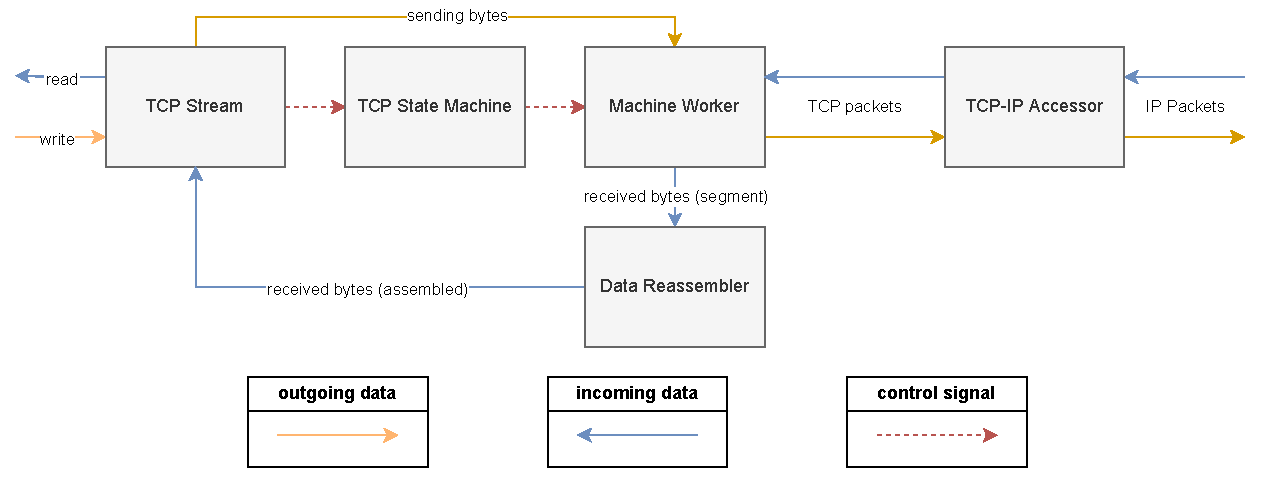
\includegraphics[width=\columnwidth]{./figures/tcpstream.pdf}}
    \caption{the structure of TCP Stream}
    \label{tcpstream}
  \end{center}
\end{figure}
\begin{figure}[H]
  \begin{center}
    \centerline{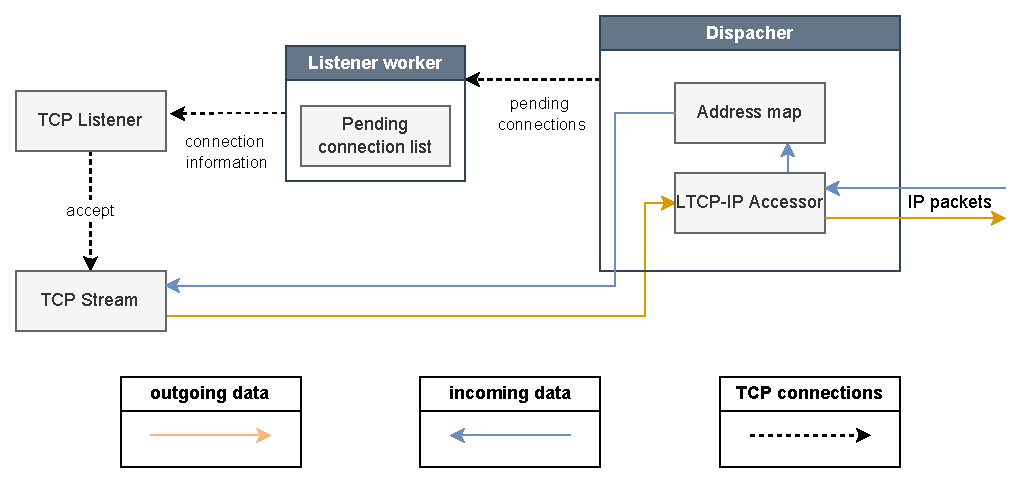
\includegraphics[width=\columnwidth]{./figures/tcplistener}}
    \caption{the structure of TCP Listener}
    \label{tcplistener}
  \end{center}
\end{figure}
As depicted in Figure~\ref{tcpstream}, TCP Stream is composed of five parts.
\begin{itemize}
  \item \textbf{TCP Stream:} The host interacts directly with the TCP Stream. TCP Stream will send the data to the Machine Worker and receive data from Data Reassembler.
  \item \textbf{TCP State Machine} will handle the control signal (such as connecting to the remote or closing the connection) from TCP Stream and send them to the Machine Worker. TCP State Machine is also responsible for releasing the resources after the host drops TCP Stream.
  \item \textbf{Machine Worker} handles the state transition of the TCP. It will also pack the data from the TCP stream, send them to the TCP-IP Accessor, unpack the incoming TCP packets, and send the unpacked bytes to Data Reassmebler.
  \item \textbf{TCP-IP Accessor} is the bridge between the network layer and the transport layer. It packs the TCP packets into IP Packets, periodically receives IP packets, and sends the unpacked TCP packets to the Machine Worker.
  \item \textbf{ Data Reassembler} receives the byte segment from the Machine Worker and reassembles them according to the TCP sequence number. The reassembled bytes will then be sent to the TCP Stream for the host to read.
\end{itemize}
\subsubsection{TCP Listener}

As shown in Figure~\ref{tcplistener}, TCP Listener is composed of three parts:
\begin{itemize}
  \item \textbf{TCP Listener} responds to the host's request. It will ask the Listener Worker for information on the incoming connection if it tries to accept a connection. The created TCP Stream will change its TCP-IP accessor to the Dispatcher.
  \item \textbf{Listener Woker} receives the connection from the Dispatcher and temporarily stores it for the TCP Listener.
  \item \textbf{Dispacher} owns an LTCP-IP Accessor to communicate with the IP server. On receiving the IP packet, it will dispatch the inner TCP packet according to its Address map. If the TCP is an SYN packet, it will create a new entry in the Address Map and send the information to the Listener Worker. On receiving TCP packets from the TCP Stream, it will pack them into IP packets and forward them to the IP server.
\end{itemize}
The TCP Listener is capable of handling multiple connections at the same time.